\chapter{Method}

This chapter will introduce and develop the \rrtfunnel\ algorithm, through two
means: Developing robust motion primitives through the \ac{SOS} programming
framework, based on the work in~\cite{majumdarFunnelLibrariesRealtime2017}, and
second deploy these funnels as motion primitives in a discrete \ac{RRT} planner,
based on~\cite{lavalleLav98cPdf}. This is beneficial, as using \textit{robust}
motion primitives has several advantages. Firstly, they are robust to
uncertainty, and thus, as long as the uncertainties in the system are akin to
our assumptions, the vehicle will not leave the funnel path. Secondly, with the
assumption that the primitives are robust, there is no need for more
conservative maneuvers and heuristics, such as maximizing the distance to an
obstacle. This means that a robust motion primitive algorithm can perform more
aggressive maneuvers than one that is inherently cautious about its
environment~\cite{majumdarFunnelLibrariesRealtime2017}.

\subsection{Simulating the funnels, checking if the model stays within the
  funnel at all times.}

\section{Distance metric for expansion (Maybe for the RRT section?)}

\section{Poisson generation of the simulated forest} (Cool section!)

\section{RRT}

\subsubsection{The identity funnel for starting the simulation fresh}

The identity funnel is an empty placeholder for the start node of the graph,
that does no transformations on the model at all, and thus can be seen as the
identity element in the funnel space, or rather, the identity funnel.

\section{FunnelGraph}

One can think of funnels computed using the machinery described in
\cite[sec~4]{majumdarFunnelLibrariesRealtime2017} as \textit{robust} motion
primitives~\cite{majumdarFunnelLibrariesRealtime2017}.

As every subfunnel (\ie{} part of a funnel), is also a funnel, funnels can be
pruned. Therefore, cutting off the end, or the beginning of a funnel, will in
fact create two new funnels. This fact can be exploited in order to create new
and shorter subfunnels for use in the \rrtfunnel{} algorithm.

\begin{figure}
  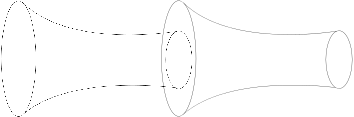
\includegraphics[scale=.2]{figures/method/funnel-composition}
  \centering
  \caption{Two funnels composed.}
\end{figure}

\section{TVLQR}

Tuning of the parameters in the \textit{TVLQR} algorithm.

\section{Simulations}

\subsection{Collision checking}

\subsection{Staying inside the funnels}

As a funnel is not simply the 2D-ellipse projected down into the plane. In fact
the funnel lives in 4D space, and as such the vehicle can leave the funnel, even
though it is inside the projected funnel in 2D space. Therefore the \rrtfunnel{}
algorithm checks at each step during the simulations that the vehicle stays
inside the verified funnels. This is done through inputting the vehicle's
current state into the quadratic Lyapunov function
\[
  {\bar{x}}^{T}S_{k}\bar{x} + \bar{x}s_{1} \bar{x} s_{2}
\]

\subsection{Expanding the size of the funnel by the size of the simulated vehicle}

The size of the vehicle in the model is in the original vehicle model in
\ref{TODO}, a single point, and as such, not accounted for in the funnel before
running simulations. Therefore the funnels have to be expanded in order for them
to accomodate the necessary robustness guarantees that are expected. However,
the size of the vehicle only affects the size of the funnel ellipsis projected
down into the xy-plane. Therefore first getting the projected size of the funnel
\[
  S_{p} = CSC^{T} (TODO - check)
\]
where
\[
  C =
  \begin{bmatrix}
    I & \mathbf{0} \\
    \mathbf{0} & \mathbf{0} \\
\end{bmatrix}
\]
and then expanding with the radii of the vehicle (TODO) using th
\[
                Sp = obj.funnels{i}.Sp{j};
                [VV,DD] = eig(Sp);
                l1 = 1/sqrt(DD(1,1)) + radius;
                l2 = 1/sqrt(DD(2,2)) + radius;
                % l3 = 1/sqrt(DD(3,3)) + radius;
                d1 = 1/l1^2;
                d2 = 1/l2^2;
                % d3 = 1/l3^2;
                D2 = diag([d1,d2]);
                Sp2 = VV*D2*VV';
                obj.funnels{i}.cS{j} = chol(Sp2);
\]

\section{Creating more motion primitives}

Although the base motion primitive library is pretty sparse, just like the
\rrtfunnel{} algorithm creates paths from stacking motion primitives, longer
motion primitives can be built \textit{for} the \rrtfunnel{} algorithm. This is
beneficial also, as it helps the algorithm expand quickly into the unsearched
parts of the searchspace, and therefore helps it regain some of the benefits of
the original \ac{RRT} algorithm.

(Downsides -- does not necessarily expand into other parts than the xy-plane).

\subsection{}

\section{Funnel-graph}

Even though the \rrtfunnel{} algorithm can work just fine with a collection of
funnels, and simply bruteforcing all funnels at the planning stage, it is
helpful to associate some kind of structure with the collection. In essence
associating the collection of funnels \(\mathcal{F}\) with some structure.
Giving the collection \(\mathcal{F}\) a tree structure, where each node in the
tree is reached, either through a funnel, a part of a funnel (which is also a
funnel), or a composition of funnels. Each funnel already has a set of nodes
associated with itself from the discretization taking place prior to funnel
creation as shown in figure \ref{fig:somefig}.

\begin{figure}
  \centering
  \begin{minipage}[b]{0.4\textwidth}
    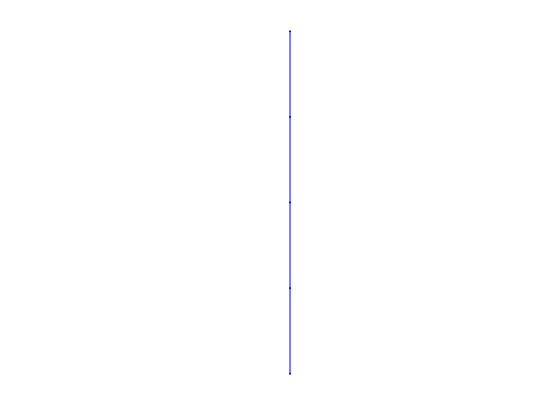
\includegraphics[width=\textwidth]{figures/method/trajectory-sampled}
    \caption{Trajectory sampled \# times (TODO)}
  \end{minipage}
  \hfill
  \begin{minipage}[b]{0.4\textwidth}
    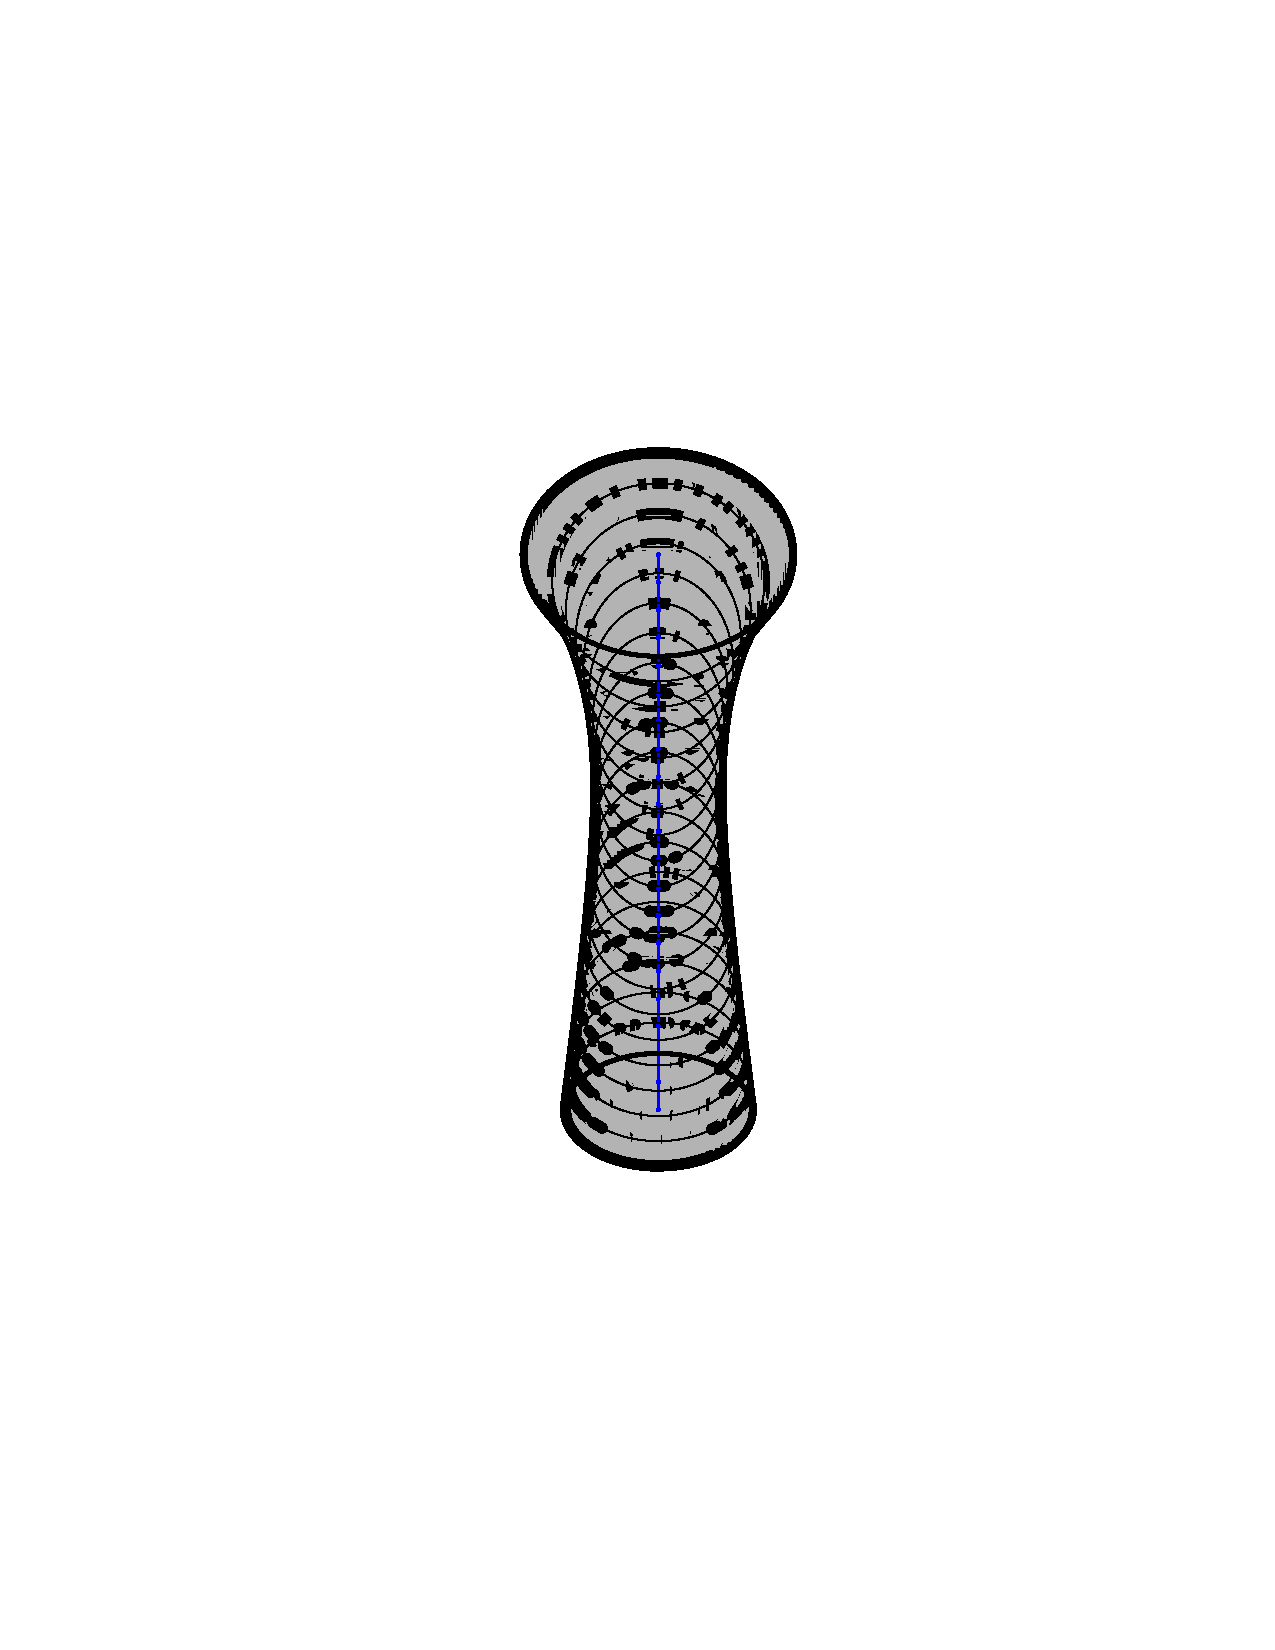
\includegraphics[width=\textwidth]{figures/method/funnel-sampled}
    \caption{The verified trajectory ellipsis overlaid at the sample times.}
  \end{minipage}
\end{figure}

For each funnel, in order to not only be able to compose funnels, but
sub-funnels, which means that at every point of every node in every funnel
composability with every other sample point in every other funnel has to be
checked. This is summed up more orderly in algorithm
\ref{alg:create-funnel-graph}, where a funnel is a vertice in the graph, and an
ordered pair of funnels \(\left( F_{i}, F_{j} \right)\) is an edge. Composition
of funnels is checked in the same way as in \ref{def:funnel-composition}.

\begin{algorithm}
  \caption{Create Funnel Graph}
  \label{alg:create-funnel-graph}
  \DontPrintSemicolon \SetAlgoNoLine

  \KwIn{\(\mathcal{F}\) -- The basis set of funnels computed around the nominal
    trajectories.} \KwOut{\(\mathcal{G}(\mathcal{F})\) -- Directed graph
    representing the composability of funnels.}

  \ForEach{\(F_{i} \in \mathcal{F}\)} { \ForEach{\(F_{j} \in \mathcal{F}\)} {
      \ForEach{\(t_{k} \in F_{i}\)} { \ForEach{\(t_{l} \in F_{j}\)} {
          \If{\(F_{i}(t_{k}) \subset F_{j}(t_{l})\)} { \(\mathcal{G}
            \leftarrow{} \left( F_{i}(t_{k}), F_{j}(t_{l}) \right)\) } \; } \; }
      \; }\; }\;

\end{algorithm}

\section{RRT-section}

